
The DATURA beam telescope is a tabletop tracker featuring six pixel detectors on aluminium rails, a Trigger and Logic Unit (TLU) providing trigger logic and time stamp information on particle passage,
 four scintillators with photo multiplier tubes (PMT) for trigger purposes, and hardware and software for data acquisition. 
Figure\,\ref{fig:datura-tscope} shows the pixel planes with its auxiliary connectors on the rails. 
A DUT is usually inserted in middle of the six planes, with three planes up- and down-stream of the DUT. 
 
\subsection{Sensors and mechanics}

Six Mimosa26 CMOS pixel detectors with $\unit{18.4}{\upmu\meter} \times \unit{18.4}{\upmu\meter}$ sized pixels arranged in 1152 columns and 576 rows
 are used for precise spacial measurement of particle trajectories.\,\cite{Mimosa26}
This adds to a total of about four million readout channels covering roughly 10\,mm times 20\,mm. 
The 350\,nm CMOS technology used for manufacture of the Mimosa26 detectors is an industry standard used in a variety of commercial applications. 
A simple two transistors/one diode approach to collect diffused charge produced in the underlying \unit{14}{\upmu\meter} epitaxial layer
 allows the construction of pixels with a pitch of less then $\unit{20}{\upmu\meter}$.
%With the rising industrial interest in high resistivity epitaxial silicon for CMOS detectors the production cost of improved noise and radiation hardness parameters
% became already possible with ~400 Ohm·cm for 10 μm epitaxial layer for Mimosa26. 
The average noise occupancy does not exceed $10^{-5}$ for non-irradiated sensors at room temperature at the signal threshold level consistent with an average efficiency above 98\,\%. 
For stable performance the detectors are kept at $\sim\unit{18}{\celsius}$. 
The readout of the Mimosa26 detectors is performed in a rolling shutter approach, which takes 16 cycles of an 80 MHz clock per row, with all 1152 columns being readout in parallel. 
The 16 clock cycles allow for correlated double sampling and zero suppression being performed on-chip with the digital circuitry placed outside of the pixel array.
At this clock frequency the Mimosa26 integration time equals $\unit{115.2}{\upmu\second}$ and allows about 8680 frames per second to be read out. 
With the on-chip buffer size being able to accommodate the data of about a few hundred pixels (above threshold) on the sensor,
the expected maximum rate of particles through the active area estimates to about $\unit{1}{\mega\hertz/\centi\meter^2}$. 

Every pixel sensor is mounted within a aluminium jigs, and three jigs are in turn are mounted on one out of two aluminium arms upstream or downstream of the DUT. 
Each arm is adjustable in the beam direction in order to ease measurements varying in DUT size.
The minimal distance of the jigs is given by the jig thickness to be 20\,mm. 
A maximal distance of 150\,mm is possible with the arms. 
Additionally, a XY$\upphi$-stage is available for translation over the acceptance region and rotation of the DUT. 
Here, the XY plane is parallel to the sensor planes, and Z points along the beam direction. 
The Mimosa26 sensors are $\unit{50}{\upmu\meter}$ thick and are protected on each side by $\unit{25}{\upmu\meter}$ thick, lightproof Kapton foil. 
Holes are machined in the jigs were the sensors sit, and hence the beam passes through, in order to minimise material budget. 
In total, this leads to a material budget of $\unit{300}{\upmu\meter}$ silicon and $\unit{300}{\upmu\meter}$ Kapton, which needs to be taken into account for electron/positron beams in the few GeV range. 

The entire tracker is placed on a rotatable frame easing the orientation parallel to the beam direction. 
Additionally, this frame is mounted on a sturdy structure providing stability over time and wheels for easy transportation. 

\begin{figure}[tb]
	\center
	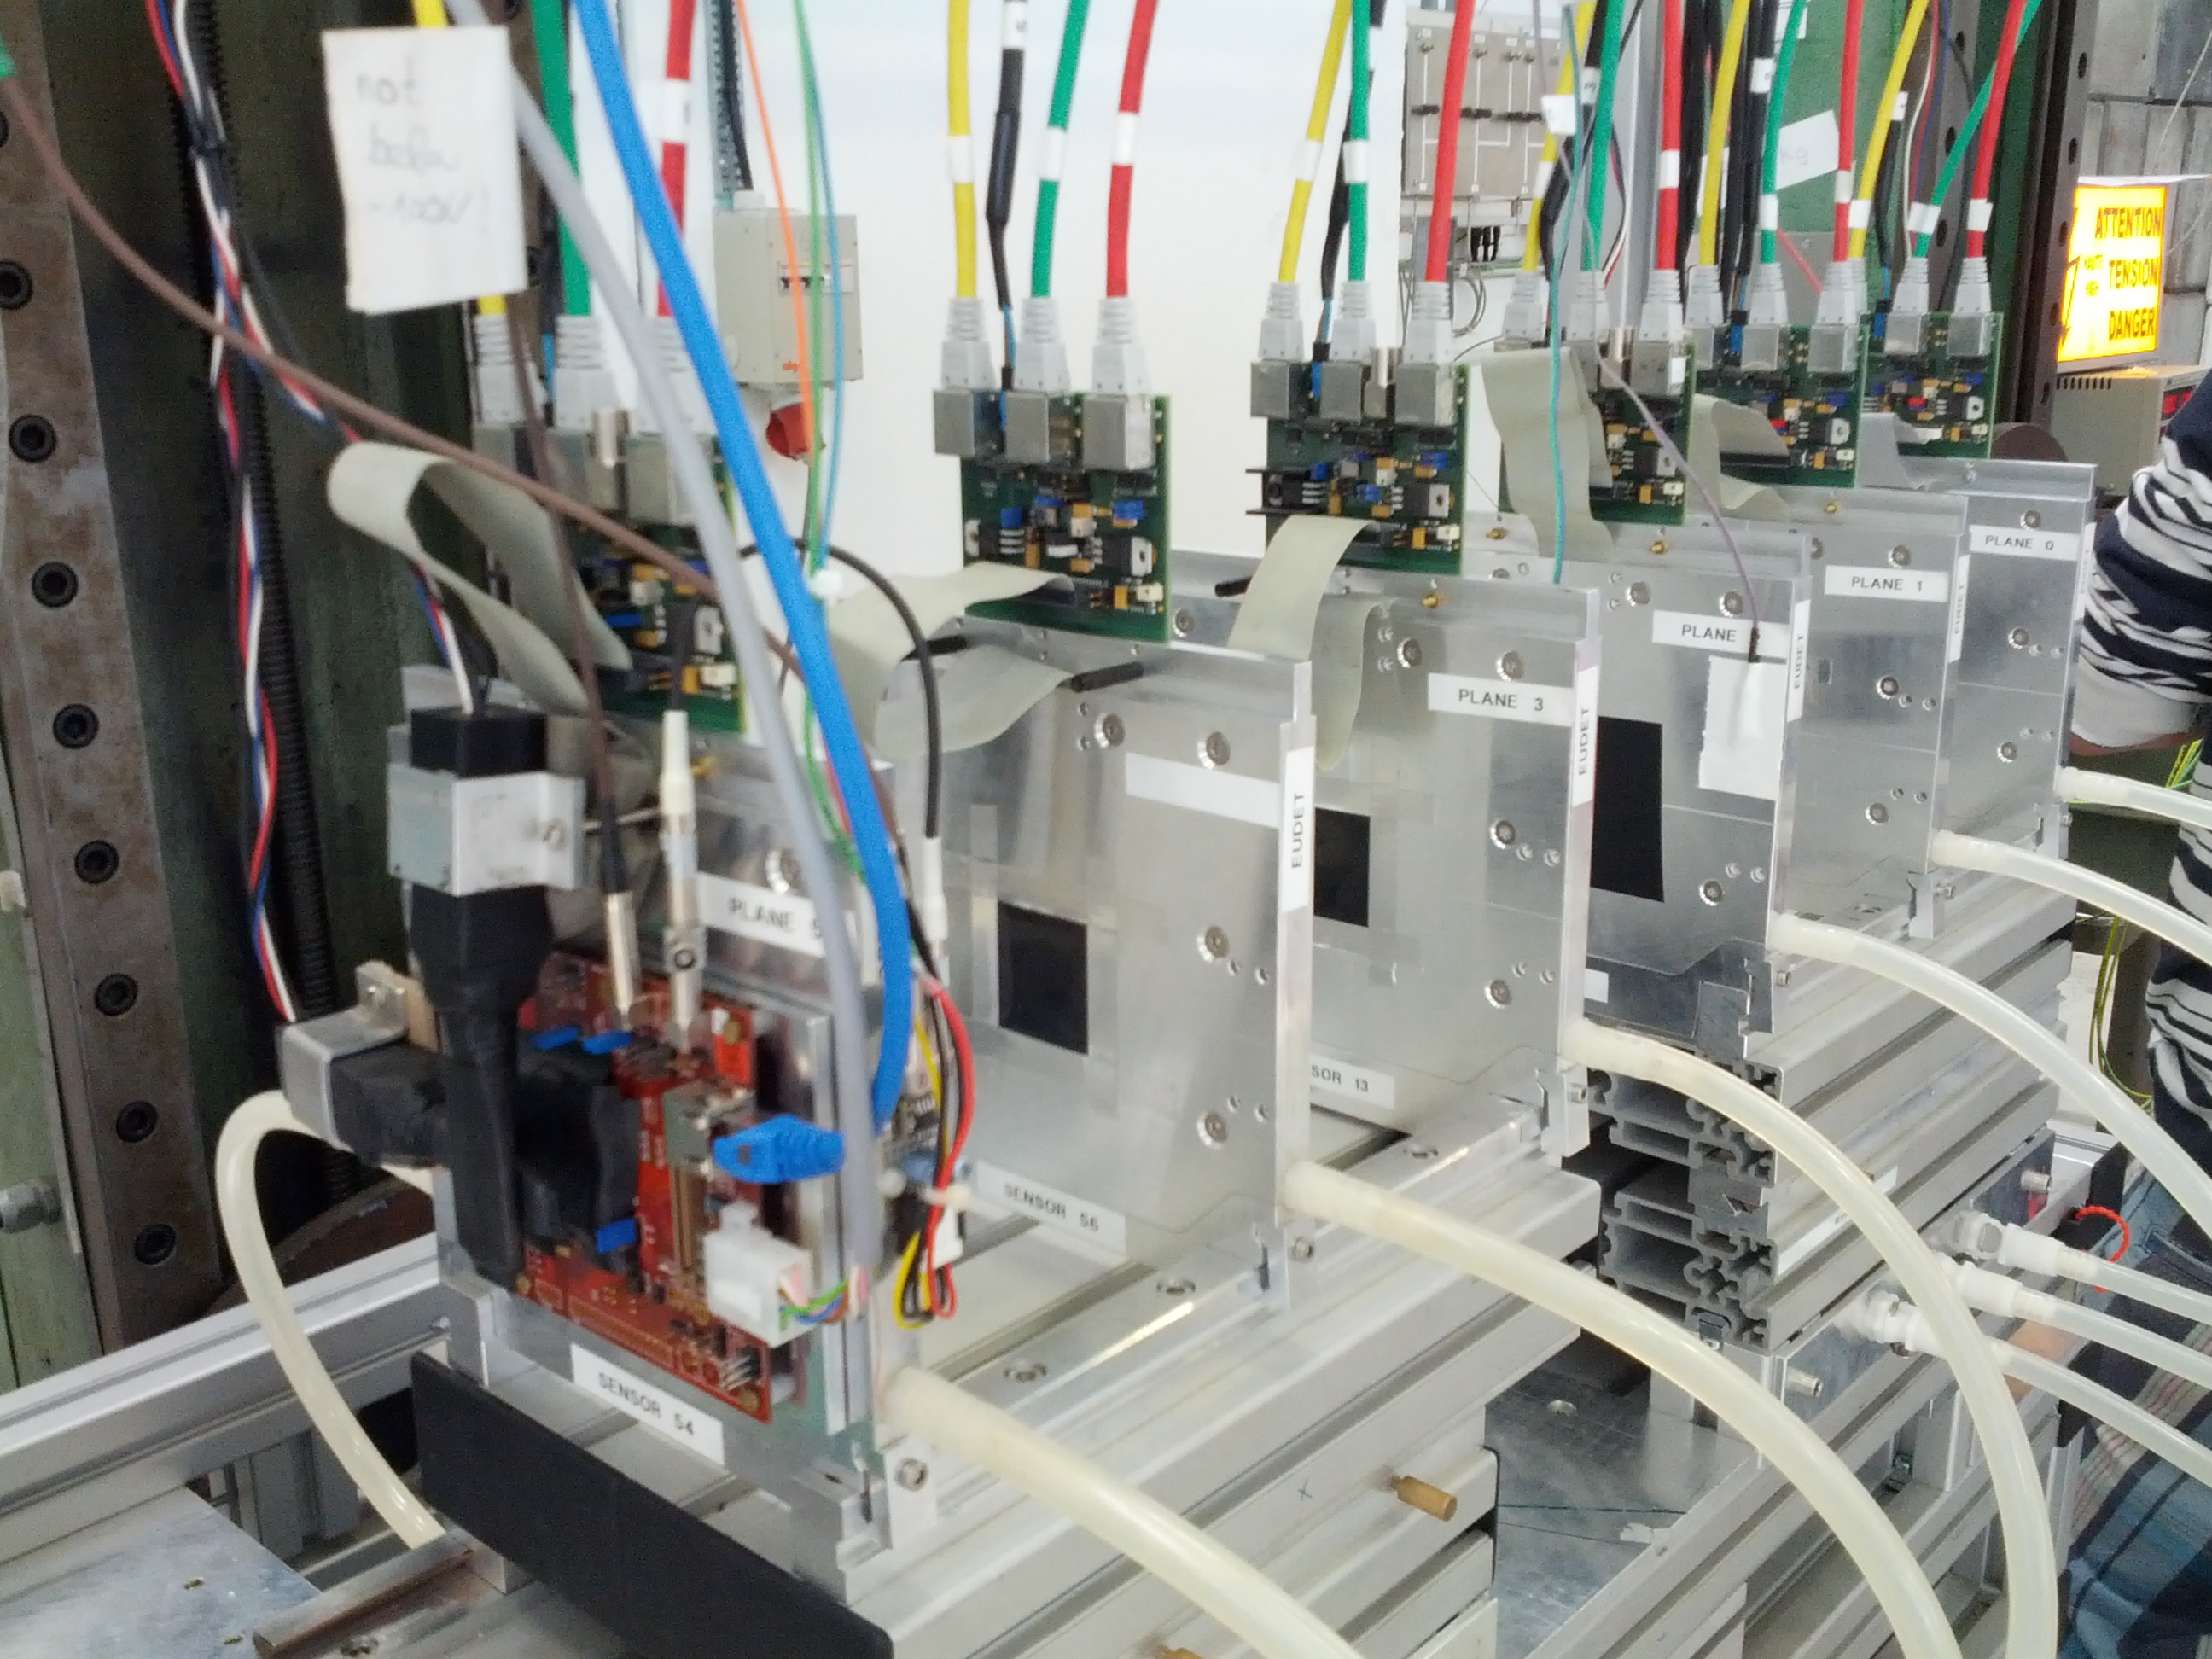
\includegraphics[width=.9\textwidth]{figures/AIDA.jpg}
	\caption[The DATURA telescope]{The DATURA telescope with its six Mimosa26 sensors on an aluminium rail is shown.}
	\label{fig:datura-tscope}
\end{figure}

!! Exchange picture with DATURA one

\subsection{Trigger and DAQ system}

Based on a commercial Spartan\,3 board, the TLU is equipped with several custom-made add-on PCBs in order to interface PMT input signals
 and attached other devices like LHC-type sensors via RJ45 connectors or LEMO connectors (NIM or TTL). 
Providing a programmable logic, the TLU  takes the trigger decision and distributes the trigger signal to all DAQ systems integrated with the telescope framework.
Four Hamamatsu PMTs assemblies with scintillators and lightguides, two in front and two in the back of the telescope, define the spatial acceptance window for triggers. 
The cross configuration of the scintillators define a rectangular acceptance window of 10\,mm times 20\,mm matching the Mimosa26 acceptance area. 
Up to four PMT signals can be used to feed the TLU. 
%The powering of the PMTs can be provided by a two channel power supply and, alternatively, by a 

From a hardware point of view, the Mimosa26 sensors provide the spatial, zero-suppressed hit data over a flat ribbon cable to so-called AUX boards, which provide RJ\,45 connectors to connect them with the
 data distribution box collecting the data from all six sensors and the TLU. 
A 52-pin cable then transports the data and the TLU information in parallel into a FlexRIO board, which is equipped with analogue-to-digital converters and an FPGA. 
If a trigger is seen by the FPGA, the data is send further to a so-called data collector, collecting the data from different DUTs. 

From a software point of view, the software integration of the DAQ systems and the TLU, together with a run control GUI, logging, data storing, and online monitoring systems are provided within the EUDAQ framework. 
EUDAQ serves as a tool set and an integration layer for DAQ systems, providing the communication protocols for them to participate in a common DAQ. 
The design of the TLU and of EUDAQ explicitly requires each DAQ system to issue a data packet readout by its detector electronics, and send it to a central data collector. 
This scheme results in only one EUDAQ event per trigger signal issued by the TLU, with no subsequent triggers recorded until all DAQ systems indicate to the TLU their availability to accept new triggers.
Therefore, this architecture limits the overall trigger rate by the DAQ system with the slowest readout cycle, which in practical applications leads to a maximum rate of few thousand particles per second. 
The variety of beam lines at CERN (PS, SPS), DESY, SLAC, Fermilab, brings also differences in the beam spill structure. 
This limits the average particle rate to below 1 kHz. 

% $\unit{}{\upmu\meter}$
